
\begin{proposition}
    Если для отображения $F:\mathbb{R}^n \to \mathbb{R}^m$, отображение $\mathrm{d}F$ всюду дифференцируемо, то второй дифференциал это билинейное отображение $\mathrm{d}^2F: \mathbb{R}^n \times \mathbb{R}^n \to \mathbb{R}^m.$
\end{proposition}
\begin{proof}
Действительно, мы сказали, что если отображение
\[
 \mathrm{d}F: \mathbb{R}^n\to \mathrm{Hom}_\mathbb{R}(\mathbb{R}^n, \mathbb{R}^m) \qquad \m{p} \mapsto (\mathrm{d}F)_{\m{p}}
\]
дифференцируемо в точке $\m{a} \in \mathbb{R}$, то мы получаем второй дифференциал $(\mathrm{d}^2F)_\m{a}$:
\[
 (\mathrm{d}^2F)_\m{a}: \mathbb{R}^n\to \mathrm{Hom}_\mathbb{R}(\mathbb{R}^n, \mathbb{R}^m), \qquad \mathbb{R}^n \ni \m{h} \mapsto (\mathrm{d}\mathrm{d}F)_\m{a}(\m{h}) \in \mathrm{Hom}(\mathbb{R}^n, \mathbb{R}^m).
\]

Согласно предыдущему предложению \ref{bil=hom}, $\mathrm{Hom}_\mathbb{R}(\mathbb{R}^n, \mathbb{R}^m)$ биективно множеству всех билинейных форм $B:\mathbb{R}^n\times \mathbb{R}^n \to \mathbb{R}^m$, \textit{т.е.,}, $\mathrm{d}^2F$ -- билинейное отображение, что и требовалось доказать.
\end{proof}











\section{Пределы}

Пусть $(\m{V}, \|\cdot\|_1)$ -- нормированное пространство, пусть $\mathcal{S} \subseteq \m{V}$ -- некоторое его подмножество, пусть $\m{v}_0$ -- точка прикосновения для $\mathcal{S}$, \ie $\m{v}_0 \in \overline{\mathcal{S}}$, и пусть $F:\mathcal{S} \to \m{W}$ некоторое отображение в нормированное пространство $(\m{W}, \|\cdot\|_2).$

\begin{definition}\label{the_main_def_of_limit}
Пусть $\m{v}_0 \notin \mathcal{S}$. Мы будем говорить, что $F(x)$ \textit{имеет предел $\m{w}_0 \in \m{W}$ при $\m{v} \in \mathcal{S}$, стремящемся к $\m{v}_0$ (или $\m{w}_0$ есть предел отображения $F$ в точке $\m{v}_0\in \overline{\mathcal{S}}$ по множеству $\mathcal{S}$}), если отображение $\overline{F}:\mathcal{S} \cup \{\m{v}_0\} \to W$, определённое условиями
    \[
     \overline{F}(\m{v}) := \begin{cases}
         F(\m{v}), & \m{v} \in \mathcal{S}, \\
         \m{w}_0, & \m{v} = \m{v}_0,
     \end{cases}
    \]
    непрерывно в точке $\m{v}_0$.
\end{definition}

В этом случае, мы пишем
\[
 \m{w}_0 := \lim_{\m{v}\to \m{v}_0, \m{v} \in \mathcal{S}} F(x).
\]

\begin{mydanger}{\bf{!}}
Если $\m{v}_0 \in \mathcal{S}$, то мы пользуемся той же терминологией и теми же обозначениями как и в случае, когда отображение $F$ непрерывно в точке $\m{v}_0$, причём $\m{w}_0:=F(\m{v}_0).$
\end{mydanger}

Вспомнив определение непрерывности и открытого множества в подмножестве, и точки прикосновения, определение предела можно переформулировать следующими двумя эквивалентными способами:

\begin{definition}
 $\lim_{\m{v}\to \m{v}_0, \m{v} \in \mathcal{S}} F(x) = \m{w}_0$ эквивалентно тому, что для любого шара $B(\m{w}_0,r) \subseteq \m{W}$ найдётся такой шар $B(\m{v}_0,\delta)$, что $F(B(\m{v}_0,\delta)\cap \mathcal{S}) \subseteq B(\m{w}_0,r)$.
\end{definition}
\begin{mydanger}{\bf{!}}
    Так как $\m{v}_0$ -- точка прикосновения, то множество $B(\m{v}_0,\delta) \cap \mathcal{S}$ никогда не пусто для любого $\delta >0$, а также октрыто в $\mathcal{S}.$
\end{mydanger}

\begin{definition}\label{def_for_cont_via_d-e}
$\lim_{\m{v}\to \m{v}_0, \m{v} \in \mathcal{S}} F(x) = \m{w}_0$ эквивалентно тому, что для каждого $\varepsilon>0$ можно найти такое $\delta >0$, что из $\m{v} \in \mathcal{S}$ и $\|\m{v} - \m{v}_0\|_1 <\delta$ следует $\|F(\m{v}) - \m{w}_0\|_2<\varepsilon.$
\end{definition}

\begin{proposition}
    Отображение может иметь лишь один предел по множеству $A$ в данной точке $a \in \overline{A}.$
\end{proposition}
\begin{proof}
    Пусть  $\lim_{x \to a, x \in A}f(x) = a'$ и  $\lim_{x \to a, x \in A}f(x) = b'$, при этом $a' \ne b'$. Тогда, согласно Определению \ref{def_for_cont_via_d-e}, 
 \begin{enumerate}
     \item  $\lim_{x \to a, x \in A}f(x) = a'$ означает, что для любого $\varepsilon >0$ можно найти такое $\delta_1 >0$, что из $x \in A$ и $d(x,a)<\delta_1$ следует $d'(a',f(x))<\varepsilon$
     \item $\lim_{x \to a, x \in A}f(x) = b'$ означает, что для того же $\varepsilon >0$ можно найти такое $\delta_2 >0$, что из $x \in A$ и $d(x,a)<\delta_2$ следует $d'(b',f(x))<\varepsilon$.
 \end{enumerate}
Тогда по неравенству треугольника
\[
 d'(a',b') \le d'(a', f(x)) + d'(f(x), b') < 2\varepsilon,
\]
\ie расстояние между фиксированными точками $a',b' \in E'$ может быть любым, что невозможно если $a' \ne b'.$
\end{proof}

Из определения предела вытекает:
\begin{theorem}[{Критерий непрерывности}]\label{criteria_of_continous_on_Rn}
Пусть $F$  -- отображение нормированных пространств $F: \m{V} \to \m{W}$. Для того чтобы $F$ было непрерывно в точке $\m{v}_0 \in \m{V}$, являющейся точкой прикосновения множества $\m{V}\setminus\{\m{v}_0\}$, необходимо и достаточно, чтобы $$F(\m{v}_0) = \lim_{\m{v} \to \m{v}_0, x\in \m{V} \setminus \{\m{v}_0\}}F(\m{v}).$$
\end{theorem}
\begin{proof}
    Это лишь пересказ определения.
\end{proof}

\begin{theorem}\label{limit_for_any_subset}
    Пусть $a' = \lim_{x \to a, x \in A} f(x)$. Тогда для каждого подмножества $B \subseteq A$, для которого $a \in \overline{B}$, $a' = \lim_{x \to a, x \in B}f(x)$.
\end{theorem}

\begin{proof}
    Это сразу следует из определения предела и следствия \ref{restriction}.
\end{proof}

\begin{theorem}\label{lim_of_composition}
    Пусть $E,E',E''$ -- метрические пространства, $A \subseteq E$, и $f:A \to E'$, $g:E' \to E''$ -- отображения. Если $\lim_{x \to a, x \in A}f(x) = a'$ и $g$ непрерывно в точке $a'$, то $g(a') = \lim_{x \to a, x \in A}g(f(x))$. 
\end{theorem}
\begin{proof}
    Это сразу следует из определения предела и теоремы \ref{comp_of_continous}.
\end{proof}

\begin{mydanger}{\bf{!}}
    В случае, когда $A = E$, мы будем вместо $\lim_{x \to a, x \in A}f(x)$  писать $\lim_{x \to a}f(x).$
\end{mydanger}

\begin{remark}
 Пусть $E = \overline{\mathbb{R}}$ -- расширенная прямая, рассмотрим выражение $$\lim_{x \to +\infty, x \in \mathbb{{R}}}f(x) = a',$$ где $f:\mathbb{R} \to E' $ - некоторое отображение. Мы знаем, что $B(+\infty, \delta) = (\frac{1-\delta}{\delta}, \infty]$. Тогда непрерывность в точке $+\infty$ означает, что для любого $r >0$ найдётся такой $\delta>0$, что $f((\frac{1-\delta}{\delta}, \infty]) \subseteq B(a',r)$. Другими словами, если $\lim_{x \to + \infty} f(x) = a'$, то для любого шара $B(a',r)$ найдётся такое число $\alpha \in \mathbb{R}$ что $f(\beta) \in B(a',r)$ для всех $\beta > \alpha.$ \textbf{Именно так мы и будем понимать запись $\lim_{x \to +\infty}f(x) = a'$};
 \[
  \boxed{ 
    \boxed{
    \lim_{x \to +\infty}f(x) = a' \Longleftrightarrow \forall r > 0\, \exists \alpha \in \mathbb{R}:\, f(\beta) \in B(a',r) \,\forall \beta >\alpha.
    }
}
 \]
\end{remark}

\begin{mydanger}{\bf{!}}
    В частности, если $E' = \mathbb{R}$ с обычной метрикой и $\mathbb{N} \subseteq \overline{\mathbb{R}}$, то $\lim_{x \to +\infty, x \in \mathbb{{N}}}f(x) =a'$ есть знакомое нам определение предела последовательности.
\end{mydanger}

\begin{lemma}\label{choice_of_seqeunce}
    Для любой точки $a \in \overline{A}$ существует такая последовательность $\{x_n\}$ точек из $A$, что $a = \lim_{n \to \infty} x_n$
\end{lemma}

\begin{proof}
    Так как $a$ -- точка замыкания, то любой шар $B(a, r)$ содержит хотя бы одну точку из $A$, \ie $B(a, r) \cap A \ne \varnothing$. В частности, для любого $n\ge 1$, $B(a, \frac{1}{n}) \cap A \ne \varnothing$. Тогда по Аксиоме Выбора, для каждого $n\ge 1$ мы можем выбрать $x_n \in B(a, \frac{1}{n})$. Покажем, что $\lim_{n \to \infty} x_n = a$. Действительно, пусть $n<m$, и мы имеем тогда $x_n \in B(a, \frac{1}{n})$, $x_m \in B(a, \frac{1}{m})$. 

    Тогда имеем
    \[
     d(x_n, x_m) \le d(a,x_n) + d(a,x_m) <\frac{1}{n} + \frac{1}{m} < \frac{2}{n}.
    \]

Это означает, что все $x_n, x_{n+1}, \ldots \in B(a, \frac{2}{n})$, что и доказывает требуемое.
\end{proof}

\begin{corollary}\label{Weirstrass_mega}
    Подмножество $F$ в метрическом пространстве $E$ замкнуто, тогда и только тогда, когда из любой последовательности $(x_n)$ в $F$, можно выбрать сходящуюся подпоследовательность $(x_{n_k})$, такую, что $\lim_{n\to \infty} x_{n_k} \in F$. 
\end{corollary}

\begin{proof}
    По Предложению \ref{closure}, $F$ замкнуто, если и только если $F = \overline{F}$. Тогда используя лемму \ref{choicе_of_seqeunce}, мы завершаем доказательство. 
\end{proof}



\begin{theorem}\label{lim=>for_any_sequence}
    Пусть $f: A \to E'$ -- отображение множества $A \subseteq E$ в метрическое пространство $E'$ и $a \in \overline{A}.$ Для того, чтобы $f$ имело предел $a' \in E'$ в точке $a$ по $A$, необходимо и достаточно, чтобы для каждой последовательности $\{s_n\}$ точек из $A$, сходящейся к $a$, последовательность $f(s  _n)$ сходилась к $a'.$
\end{theorem}

\begin{proof}~

(1) Необходимость. 

Пусть $\lim_{x \to a, x \in A}f(x) = a'$, и пусть $s:\mathbb{N} \to {A}\cup \{a\}$ -- последовательность $\{s_n\}$. По условию, $\lim_{n \to \infty }s_n = a$ и так как $\lim_{x \to a, x \in A}f(x) = a'$, то по определению предела \ref{thе_main_def_of_limit}, $\overline{f}$ непрерывна в точке $a$. Тогда по Теореме \ref{lim_of_composition}, последовательность $s':=\overline{f} \circ s: \mathbb{N} \to E'$, в которой $s'_n = f(s_n)$, имеет предел $\overline{f}(a) = a'$, что и доказывает необходимость.

(2) Достаточность.

Будем доказывать от противного. Пусть для любой последовательности $\{s_n\}$ точек из $A$, $\lim_{n \to \infty} s_n = a$ имеем $\lim_{n \to \infty}f(s_n) = a'$, но $a' \ne \lim_{x \to a, x\in A}f(x).$ Тогда  $\lim_{n \to \infty} s_n = a$ влечёт, что, начиная с какого-то номера $N$, $d(a,s_n) < \varepsilon$ для всех $n > N$.

С другой стороны, $a' \ne \lim_{x \to a, x\in A}f(x)$ означает, что $f(x)$ не является непрерывным в точке $a$. Тогда, существует такое $\varepsilon >0$, что для любого номера $n$ найдётся такая точка $x_n \in A$, удовлетворяющая двум условиям: $d(a,x_n) < \frac{1}{n}$ и $d'(a',f(x_n))\ge \varepsilon$. Но тогда последовательность $\{f(s_n)\}$ не сходится к $f(s)$, что противоречит условию.
\end{proof}


\begin{theorem}\label{f<g=>lim}
  Пусть $E$ -- метрическое пространство с метрикой $d$, и $\mathbb{R}$ -- рассматривается с обычной метрикой $d'(x,y): = |x-y|$.  Пусть $f,g:A \to \mathbb{R}$ -- функции такие что $f(x) \le g(x)$ для всех $x \in A$, тогда $\lim_{x\in A, x \to a}f(x) \le \lim_{x \in A, x \to a}g(x)$.
\end{theorem}

\begin{proof}
Пусть $\lim_{x\in A, x \to a}f(x) = \alpha$, $\lim_{x\in A, x \to a}g(x) = \beta$.

Тогда, по арифметике предела $\lim_{x\in A, x \to a}(g(x) - f(x)) = \beta - \alpha.$

Пусть $\alpha > \beta$. Пусть $\varepsilon : = \alpha - \beta$, тогда $\varepsilon >0$.

Из определения предела следует, что для выбранного $\varepsilon$, можно найти такое $\delta>0$, что из $d(x,a)<\delta$ будет следовать $|g(x) - f(x) - (\beta - \alpha)| < \varepsilon$, но тогда получаем, что
\[
 g(x) - f(x) < \varepsilon + (\beta - \alpha) = 0,
\]
что даёт противоречие. Это и доказывает утверждение.
\end{proof}






\section{Подпространства метрического пространства}

Пусть $F \subseteq \m{V}$ -- непустое подмножество нормированного пространства $\m{V}$, тогда $F \times F \subseteq E \times E$ -- непустое подмножество, тогда мы имеем следующую коммутативную диаграмму

\[
  \begin{tikzcd}
    F \times F \arrow[hook]{d}[left]{\mathrm{in}} \arrow{dr}{d|_{F \times F}} &  \\
    E \times E \arrow{r}[below]{d} & \mathbb{R}
  \end{tikzcd}
\]
\ie, \textit{сужая} метрику $d$ на $F$, мы получаем метрическое пространство $(F,d|_{F \times F})$, которое мы будем для простоты обозначать $(F, d_F)$.

\begin{definition}
    Метрическое пространство, определённое таким образом, называется \textit{подпространством} $F$ метрического пространства $E$.
\end{definition}

\begin{figure}[h!]
    \centering
    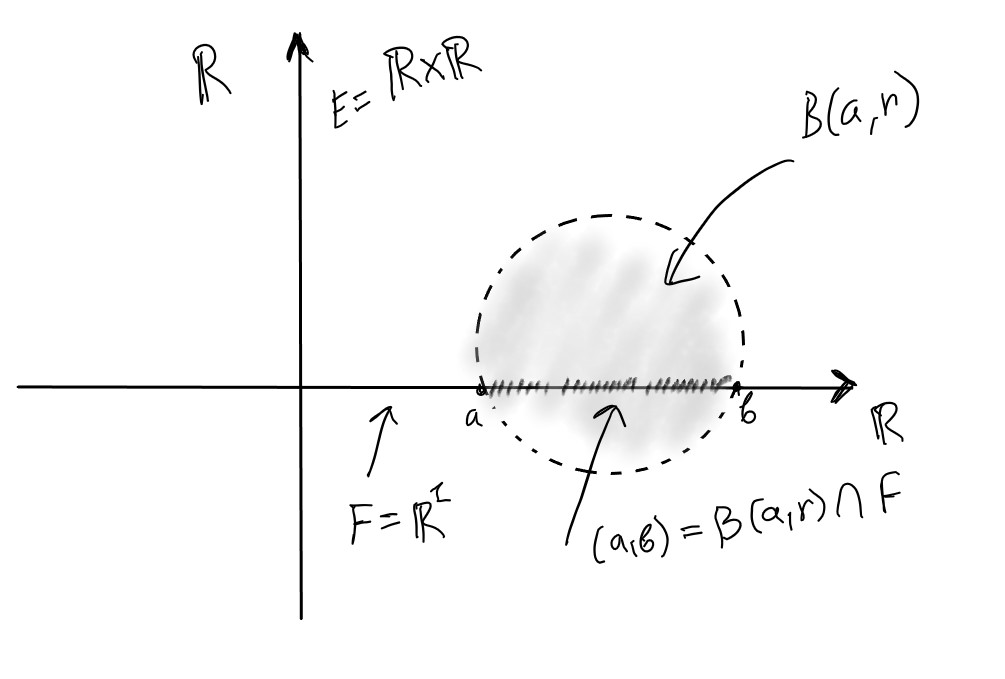
\includegraphics[scale = 0.4]{images/open_in_F.jpg}
    \caption{Пусть $E = \mathbb{R} \times \mathbb{R}$ -- обыкновенная плоскость с обыкновенной евклидовой метрикой $d(\m{x},\m{y}) = \sqrt{(x_1 - y_1)^2+ (x_2 - y_2)^2}$, и пусть $F = \mathbb{R}$, которую мы можем понимать как множество вида $\{(x,0), x\in \mathbb{R}\}$. На рисунке $F$ отождествлена с осью $Ox$. Тогда, сужая метрику $d$ на $F$, мы получаем, что $d(x,y) = \sqrt{(x-y)^2} = |x-y|$. Более того, ясно, что любой интервал $(a,b)$ можно получить, пересекая открытый круг с $F.$}
    \label{fig:enter-label}
\end{figure}


\begin{proposition}\label{open_in_subset}
    Для того чтобы множество $S \subseteq F$ было открыто в подпространстве $F$, необходимо и достаточно, чтобы существовало такое множество $\mathscr{U}$, открытое в $E$, что $S = \mathscr{U} \cap F.$
\end{proposition}

\begin{proof}
    Прежде всего, поймём, что есть открытый шар в $F$. Пусть $a \in F$, и рассмотрим открытый шар $B(a,r) \subseteq E$, тогда получаем
    \begin{eqnarray*}
        F \cap B(a,r) &:=& \{x \in E \cap F\, :\, d(x,a)<r\} \\
        &=&\{x\in F\, :\, d(x,a)<r\} \\
        &=& \{x \in F\, :\, d_F(x,a)<r\},
    \end{eqnarray*}
    \ie $F \cap B(a,r)$ -- это \textbf{открытый шар в $F$ с центром в точке $a$ радиуса $r.$}

\begin{mydanger}{\bf{!}}
    Обратим внимание, что если $F = \mathbb{R}_{\ge 0} \subseteq \mathbb{R} = E$, $d(x,y) = |x-y|$, то, например, $[0,1)$ -- открытый шар в $F = \mathbb{R}_{\ge 0}$, так как $[0,1) = (-1,1) \cap \mathbb{R}_{\ge 0}$. Hо! В $\mathbb{R}$, $[0,1)$ и не открыт и не замкнут!
\end{mydanger}

(1) Пусть $\mathscr{U}$ -- открытое множество в $E$, и пусть $x \in \mathscr{U} \cap F$. Так как $\mathscr{U}$ -- открытое в $E$, то найдётся шар $B(x,r) \subseteq E$ такой, что $B(x,r) \subseteq \mathscr{U}$. Тогда $F \cap B(x,r) \subseteq F \cup \mathscr{U}$. Но мы уже поняли, что $B(x,r) \cap F$ -- открытый шар в $F$, но тогда включение $F \cap B(x,r) \subseteq F \cup \mathscr{U}$ и означает, что $\mathscr{U} \cap F$ открыто в $F$, ибо $x$ -- произвольная точка в $\mathscr{U} \cap F.$

(2) Пусть $S$ открыто в $F$, это значит, что для любой точки $x \in S$ можно найти открытый шар $B(x, r(x)) \subseteq E$ такой, что $F \cap B(x,r(x)) \subseteq S$ (т.к., $F \cap B(x,r(x))$ -- это открытый шар в $F$).

Тогда 
\[
 S = \bigcup_{x \in S} F \cap B(x, r(x)) = F \cap \mathscr{U},
\]
где $\mathscr{U} = \cup_{x\in S} B(x, r(x)) \subseteq E$, тогда по Леммам \ref{open_ball=open}, \ref{union_and_cap_of_open} $\mathscr{U}$ открыто в $E$.
\end{proof}








\section{Сходимость в $\mathbb{R}^n$}



Для доказательства обобщённой теоремы Больцано--Вейерштрасса и вообще в дальнейшем нам понадобится следующее неравенство

\begin{lemma}\label{m<d<M}
Для любых $x_1,\ldots, x_n \in \mathbb{R}$ 
\[
\max_{1 \le k \le n} |x_k| \le \sqrt{\sum_{k=1}^n x_k^2} \le \sqrt{n} \max_{1\le k \le n} |x_k|.
\]
\end{lemma}
\begin{proof}
 
Действительно, перенумеруем все $x_i$ так, чтобы $x_1^2 \le x_2^2 \le \ldots \le x_n^2$, \ie $\max_{1 \le k \le n} |x_k| = x_n$. Но тогда получаем
\[
 \sqrt{x_1^1 + \cdots + x_n^2} \le n x_n^2, 
\]
и 
\[
 x_n^2 \le \sqrt{x_1^1 + \cdots + x_n^2},
\]
что и даёт требуемое неравенство.    
\end{proof}

Для любого вектора $\m{v} = (v_1,\ldots, v_n)^\top \in \mathbb{R}^n$, мы положим 
\[
 \| \m{v} \| : = \sqrt{ v_1^ + \cdots + v^n},
\]
это число называют \textit{нормой} или \textit{длиной} вектора $\m{v}.$




Зафиксируем обозначения. Для каждого элемента $\m{x}_m$ последовательности $\{\m{x}\}$, положим $\m{x}_m = (x_{1m}, x_{2m}, \ldots, x_{nm})^\top$ для каждого $m \ge 1$. Таким образом, всю последовательность можно представить в виде бесконечной матрицы
   \[
    \m{x} = (\m{x}_1,\ldots, \m{x}_m, \ldots,) = \begin{pmatrix}
        x_{11} & x_{12} & \ldots & x_{1m} & \ldots \\
        x_{21} & x_{22} & \ldots & x_{2m} & \ldots \\
        \vdots & \vdots & \ddots & \vdots & \ddots \\
        x_{n1} & x_{n2} & \ldots & x_{nm} & \ldots
    \end{pmatrix}
   \]

\begin{lemma}
    Если $(\m{x}_m)$ последовательность в $\mathbb{R}^n$ такая, что $\lim_{m \to \infty}\m{x}_m = \m{a}$, то она сходится по координатно, \ie $\lim_{m\to \infty}x_{km} = a_k$, где $\m{a} = (a_1, \ldots, a_n)^\top.$
\end{lemma}

\begin{proof}
Согласно неравенству (\ref{m<d<M}) для каждого $1 \le k \le n$, $|x_{km} - a_k| \le d(\m{x}_m, \m{a})<r$.

Имеем 
    \begin{eqnarray*}
        \lim_{m \to \infty} \m{x}_m = \m{a} &\Longleftrightarrow& \forall \varepsilon >0 \, \exists M : \forall m >M, \, d(\m{x}_m, \m{a}) = ||\m{x}_m - \m{a}|| < \varepsilon \\
        &\Longleftrightarrow& \forall\, 1 \le k \le n,\, |x_{km} - a_k| < \varepsilon \\
        &\Longleftrightarrow & \lim_{m \to \infty}x_{km} = a_k,\, 1 \le k \le n,
    \end{eqnarray*}
    что доказывает требуемое.
\end{proof}


\begin{theorem}[\textbf{Обобщённая теорема Больцано--Вейерштрасса}]\label{genB-W}
    Рассмотрим $\mathbb{R}^n$ с обычной метрикой $d$, и пусть имеется такая последовательность $\{\m{x}_m\}$, элементы которой целиком лежат в каком-то шаре $B(\m{a},r)\subseteq \mathbb{R}^n$, тогда в ней имеется сходящаяся подпоследовательность.
\end{theorem}
\begin{proof}

    Пусть $\{\m{x}_m\} \subseteq B(\m{a},r)$, тогда $d(\m{x}_m, \m{a})<r$, но тогда согласно (\ref{m<d<M}),
    \[
     |x_{km} - a_k| \le \max_{1\le k \le n}| x_{km} - a_{k}  | \le d(\m{x}_m, \m{a})<r,
    \]

Так как $\m{a} =(a_1,\ldots, a_n)^\top$ --- фиксированная точка, то числовая последовательность $\{x_{km}\}$ ограничена при каждом $m$ и каждом $1\le k \le n$. Тогда по теореме Больцано--Вейерштрасса (Теорема \ref{B-W}) в последовательности $(x_{1m})$ можно найти сходящуюся подпоследовательность $(x_{1m_{t1}}) \subseteq (x_{1m})$, где $t_1$ пробегает какое-то множество индексов $T_1$. Рассмотрим теперь подпоследовательность $(x_{2m_{t_1}})$ последовательности $(x_{2m})$, которая также ограничена, значит, в ней можно найти сходящуюся подпоследовательность $(x_{2m_{t_2}})$, где $t_2$ пробегает какое-то множество индексов $T_2 \subseteq T_1$. Продолжая таким образом, мы в итоге получим набор подпоследовательностей
\[
 \{(x_{1m_{t_1}}), (x_{2m_{t_2}}), \ldots, (x_{nm_{t_n}})\},
\]
где каждый $t_k$ пробегает множество индексов $T_k$, при этом $T_n \subseteq T_{n-1} \subseteq \cdots \subseteq T_2 \subseteq T_1.$

Тогда положим 
\[
  \m{x}' = \begin{pmatrix}
      (x_{1m_{t_n}}) \\
      (x_{2m_{t_n}}) \\
      \vdots \\
      (x_{nm_{t_n}})
  \end{pmatrix},
\]
что и будет сходящейся подпоследовательностью.    
\end{proof}

